\documentclass[]{jarticle}          % 一段組
%\documentclass[twocolumn]{jarticle} % 二段組

\textwidth 180mm
\textheight 255mm
\oddsidemargin -12mm
\topmargin -15mm
\columnsep 10mm

%\vspace{0.5cm} % 一段組の場合はコメントアウトした方が体裁がよいx
%] % 一段組の場合はコメントアウトする

\usepackage{styles/labheadings}
\usepackage[dvipdfmx]{graphicx,color}
\usepackage{amsmath,amssymb}
\usepackage{url}
% 追加
\usepackage{listings,jvlisting}
\usepackage[hang,small,bf]{caption}
\usepackage[subrefformat=parens]{subcaption}
\captionsetup{compatibility=false}

\newcommand{\aU}{\mbox{\boldmath $a$}}
\newcommand{\bU}{\mbox{\boldmath $b$}}
\newcommand{\cU}{\mbox{\boldmath $c$}}
\newcommand{\dU}{\mbox{\boldmath $d$}}
\newcommand{\eU}{\mbox{\boldmath $e$}}
\newcommand{\fU}{\mbox{\boldmath $f$}}
\newcommand{\gU}{\mbox{\boldmath $g$}}
\newcommand{\hU}{\mbox{\boldmath $h$}}
\newcommand{\iU}{\mbox{\boldmath $i$}}
\newcommand{\jU}{\mbox{\boldmath $j$}}
\newcommand{\kU}{\mbox{\boldmath $k$}}
\newcommand{\lU}{\mbox{\boldmath $l$}}
\newcommand{\mU}{\mbox{\boldmath $m$}}
\newcommand{\nU}{\mbox{\boldmath $n$}}
\newcommand{\oU}{\mbox{\boldmath $o$}}
\newcommand{\pU}{\mbox{\boldmath $p$}}
\newcommand{\qU}{\mbox{\boldmath $q$}}
\newcommand{\rU}{\mbox{\boldmath $r$}}
\newcommand{\sU}{\mbox{\boldmath $s$}}
\newcommand{\tU}{\mbox{\boldmath $t$}}
\newcommand{\uU}{\mbox{\boldmath $u$}}
\newcommand{\vU}{\mbox{\boldmath $v$}}
\newcommand{\wU}{\mbox{\boldmath $w$}}
\newcommand{\xU}{\mbox{\boldmath $x$}}
\newcommand{\yU}{\mbox{\boldmath $y$}}
\newcommand{\zU}{\mbox{\boldmath $z$}}
\newcommand{\AU}{\mbox{\boldmath $A$}}
\newcommand{\BU}{\mbox{\boldmath $B$}}
\newcommand{\CU}{\mbox{\boldmath $C$}}
\newcommand{\DU}{\mbox{\boldmath $D$}}
\newcommand{\EU}{\mbox{\boldmath $E$}}
\newcommand{\FU}{\mbox{\boldmath $F$}}
\newcommand{\GU}{\mbox{\boldmath $G$}}
\newcommand{\HU}{\mbox{\boldmath $H$}}
\newcommand{\IU}{\mbox{\boldmath $I$}}
\newcommand{\JU}{\mbox{\boldmath $J$}}
\newcommand{\KU}{\mbox{\boldmath $K$}}
\newcommand{\LU}{\mbox{\boldmath $L$}}
\newcommand{\MU}{\mbox{\boldmath $M$}}
\newcommand{\NU}{\mbox{\boldmath $N$}}
\newcommand{\OU}{\mbox{\boldmath $O$}}
\newcommand{\PU}{\mbox{\boldmath $P$}}
\newcommand{\QU}{\mbox{\boldmath $Q$}}
\newcommand{\RU}{\mbox{\boldmath $R$}}
\newcommand{\SU}{\mbox{\boldmath $S$}}
\newcommand{\TU}{\mbox{\boldmath $T$}}
\newcommand{\UU}{\mbox{\boldmath $U$}}
\newcommand{\VU}{\mbox{\boldmath $V$}}
\newcommand{\WU}{\mbox{\boldmath $W$}}
\newcommand{\XU}{\mbox{\boldmath $X$}}
\newcommand{\YU}{\mbox{\boldmath $Y$}}
\newcommand{\ZU}{\mbox{\boldmath $Z$}}
\newcommand{\epU}{\mbox{\boldmath $\epsilon$}}
\newcommand{\taU}{\mbox{\boldmath $\tau$}}
\newcommand{\etU}{\mbox{\boldmath $\eta$}}
\newcommand{\xiU}{\mbox{\boldmath $\xi$}}
\newcommand{\wwU}{\mbox{\boldmath $\omega$}}
\newcommand{\WwU}{\mbox{\boldmath $\Omega$}}
\newcommand{\lmU}{\mbox{\boldmath $\lambda$}}
\newcommand{\LmU}{\mbox{\boldmath $\Lambda$}}
\newcommand{\PiU}{\mbox{\boldmath $\Pi$}}
\newcommand{\SgU}{\mbox{\boldmath $\Sigma$}}
\newcommand{\thU}{\mbox{\boldmath $\theta$}}
\newcommand{\ThU}{\mbox{\boldmath $\Theta$}}
\newcommand{\roU}{\mbox{\boldmath $\rho$}}
\newcommand{\nuU}{\mbox{\boldmath $\nu$}}
\newcommand{\ones}{{\bf 1}}
\newcommand{\zr}{{\bf 0}}
\newcommand{\eq}{\begin{equation}}
\newcommand{\en}{\end{equation}}
\newcommand{\eqa}{\begin{eqnarray}}
\newcommand{\ena}{\end{eqnarray}}
\newcommand{\xx}{\makebox[1cm]{}}
\newcommand{\xm}{\makebox[0.5cm]{}}
\newcommand{\x}{\makebox[0.2cm]{}}
\newcommand{\tr}{{\rm tr}}
\newcommand{\sgn}{{\rm sgn}}
\newcommand{\ad}{{\rm ad}}

\newcommand{\rank}{{\rm rank}}
\newcommand{\diag}{{\rm diag}}
\newcommand{\lbr}{\left(\begin{array}}
\newcommand{\rbr}{\end{array}\right)}
\newcommand{\Proof}{\noindent{\em Proof\/}}
\newcommand{\Solution}{\noindent{\em Solution}}
\newcommand{\Derivation}{\noindent{\em Derivation}}
\newcommand{\msp}{\vspace*{\medskipamount}\\}
\newcommand{\qed}{\hspace*{\fill}$\Box$}
\newcommand{\aX}{{\bf a}}
\newcommand{\bX}{{\bf b}}
\newcommand{\cX}{{\bf c}}
\newcommand{\dX}{{\bf d}}
\newcommand{\eX}{{\bf e}}
\newcommand{\fX}{{\bf f}}
\newcommand{\gX}{{\bf g}}
\newcommand{\hX}{{\bf h}}
\newcommand{\iX}{{\bf i}}
\newcommand{\jX}{{\bf j}}
\newcommand{\kX}{{\bf k}}
\newcommand{\lX}{{\bf l}}
\newcommand{\mX}{{\bf m}}
\newcommand{\nX}{{\bf n}}
\newcommand{\oX}{{\bf o}}
\newcommand{\pX}{{\bf p}}
\newcommand{\qX}{{\bf q}}
\newcommand{\rX}{{\bf r}}
\newcommand{\sX}{{\bf s}}
\newcommand{\tX}{{\bf t}}
\newcommand{\uX}{{\bf u}}
\newcommand{\vX}{{\bf v}}
\newcommand{\wX}{{\bf w}}
\newcommand{\xX}{{\bf x}}
\newcommand{\yX}{{\bf y}}
\newcommand{\zX}{{\bf z}}
\newcommand{\AX}{{\bf A}}
\newcommand{\BX}{{\bf B}}
\newcommand{\CX}{{\bf C}}
\newcommand{\DX}{{\bf D}}
\newcommand{\EX}{{\bf E}}
\newcommand{\FX}{{\bf F}}
\newcommand{\GX}{{\bf G}}
\newcommand{\HX}{{\bf H}}
\newcommand{\IX}{{\bf I}}
\newcommand{\JX}{{\bf J}}
\newcommand{\KX}{{\bf K}}
\newcommand{\LX}{{\bf L}}
\newcommand{\MX}{{\bf M}}
\newcommand{\NX}{{\bf N}}
\newcommand{\OX}{{\bf O}}
\newcommand{\PX}{{\bf P}}
\newcommand{\QX}{{\bf Q}}
\newcommand{\RX}{{\bf R}}
\newcommand{\SX}{{\bf S}}
\newcommand{\TX}{{\bf T}}
\newcommand{\UX}{{\bf U}}
\newcommand{\VX}{{\bf V}}
\newcommand{\WX}{{\bf W}}
\newcommand{\XX}{{\bf X}}
\newcommand{\YX}{{\bf Y}}
\newcommand{\ZX}{{\bf Z}}

% report.texと同じディレクトリにnumerical_definition.texを入れておけば上の書き方でもいいはずです

\usepackage[
  dvipdfm,
  bookmarks=true,
  bookmarksnumbered=true,
  colorlinks=true]{hyperref}
\AtBeginDvi{\special{pdf:tounicode EUC-UCS2}}

%ここからソースコードの表示に関する設定
\lstset{
  basicstyle={\ttfamily},
  identifierstyle={\small},
  commentstyle={\smallitshape},
  keywordstyle={\small\bfseries},
  ndkeywordstyle={\small},
  stringstyle={\small\ttfamily},
  frame={tb},
  breaklines=true,
  columns=[l]{fullflexible},
  numbers=left,
  xrightmargin=0zw,
  xleftmargin=3zw,
  numberstyle={\scriptsize},
  stepnumber=1,
  numbersep=1zw,
  lineskip=-0.5ex
}
%ここまでソースコードの表示に関する設定

\pagestyle{labheadings}
\headerleft{進捗報告}   % ヘッダの左側のタイトル
\headerright{2023年10月10日}  % ヘッダの右側のタイトル

\begin{document}

%\twocolumn % 一段組の場合はコメントアウトする

\vspace*{2ex}
\begin{center}
 {\Large \bf 研究の進捗と後期の目標・計画}\\ % タイトル
 \vspace*{5mm}
 {\large B4 田川幸汰}% 発表者名
\end{center}

%\vspace{0.5cm} % 一段組の場合はコメントアウトした方が体裁がよいx
%] % 一段組の場合はコメントアウトする

%新しく作成したコマンド
% \newcommand{\reffig}[1]{\hyperref[#1]{図\ref{#1}}}
% \newcommand{\refeq}[1]{\hyperref[#1]{式(\ref{#1})}}
% \newcommand{\reftab}[1]{\hyperref[#1]{表\ref{#1}}}
% \newcommand{\refsec}[1]{\hyperref[#1]{\ref{#1}章}}
% \newcommand{\refsubsec}[1]{\hyperref[#1]{\ref{#1}節}}

% 数式
%\begin{equation}
%  数式記述  
%  \label{ラベル名}
%\end{equation}

% 図
% \begin{figure}[!ht]
%   \begin{center}
%     \includegraphics[scale=0.5]{figures/画像ファイル名}
%     \caption{キャプション名}
%     \label{ラベル名}
%   \end{center}
% \end{figure}

% リスト
% \begin{enumerate or itemize}
%   \item 
% \end{enumerate or itemize}

\section{概要}
マスク有顔画像から、マスク無顔画像を生成する研究の最終目的が、現時点でどのくらい達成できたかを報告する。
また、後期の目標と計画についても報告する。

\section{マスク有顔画像から、マスク無顔画像を生成}
マスクあり顔画像からマスクなし顔画像をリアルタイムで生成する。
内容は大きく分けて三次元モデルの自動生成、マスクあり顔画像から特徴点を抽出しカメラの位置姿勢を計算、計算したカメラの位置姿勢を基にマスクなし画像を生成の三つに分類される。
以下の節では、それぞれの内容について説明する。
\subsection{三次元モデルの生成}
テクスチャ画像を入力することで三次元モデルを作成するプログラムを資料\cite{bib_1}を参考にしながら作成した。
プログラムでは、テクスチャ画像の特徴量をGoogle MediapipeのfaceMeshによって求め、その値を世界座標系に合うようにスケーリングし、三次元モデルを自動生成する。
入力したテクスチャ画像を\hyperref[one]{図\ref{one}}に示す。プログラムにより自動生成された三次元モデルを\hyperref[two]{図\ref{two}}に示す。
\begin{figure}[!ht]
  \begin{tabular}{cc}
    \begin{minipage}[t]{0.45\hsize}
      \centering
      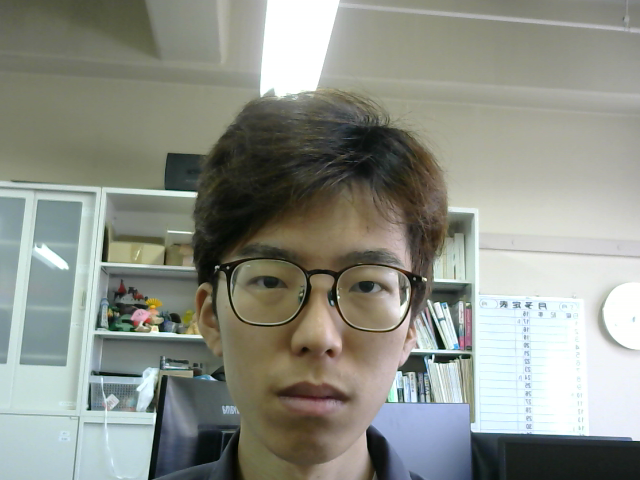
\includegraphics[keepaspectratio, scale=0.27]{figures/texture.png}
      \caption{テクスチャ画像}
      \label{one}
    \end{minipage} &
    \begin{minipage}[t]{0.45\hsize}
      \centering
      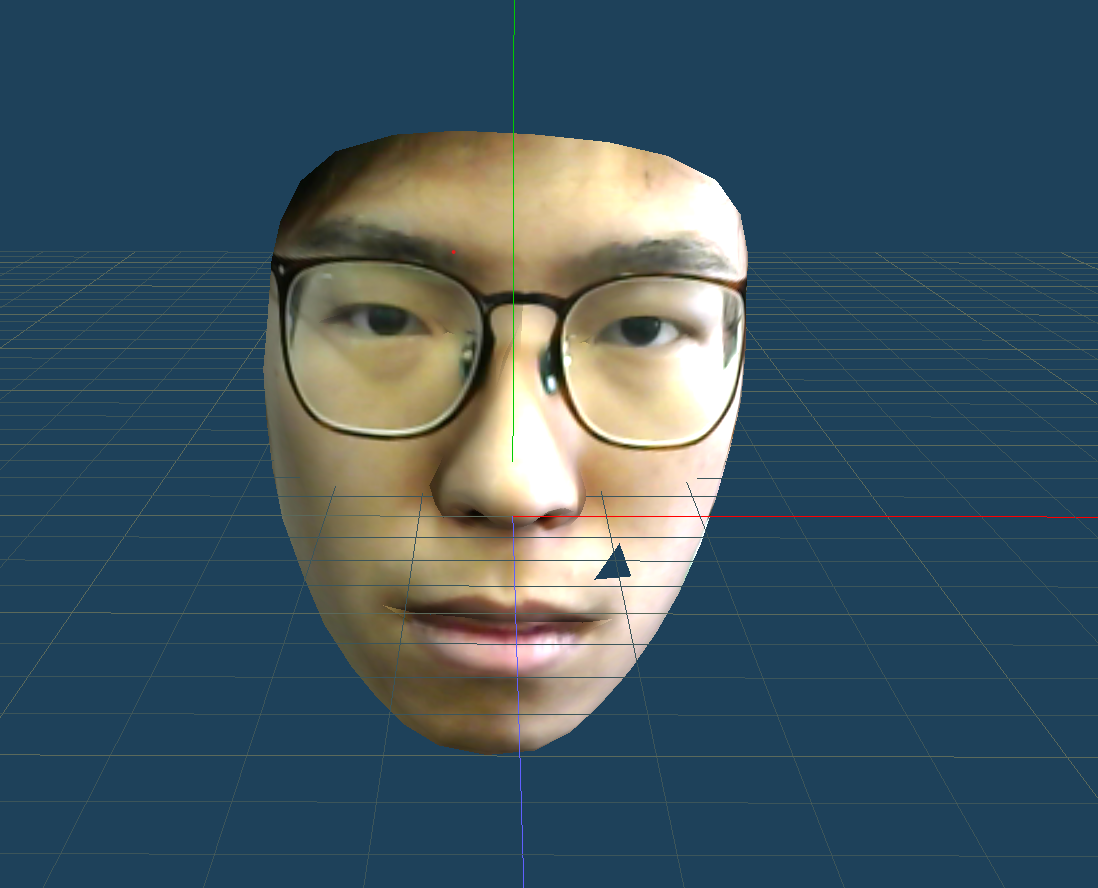
\includegraphics[keepaspectratio, scale=0.2]{figures/3dmodel.png}
      \caption{三次元モデル}
      \label{two}
    \end{minipage}
  \end{tabular}
\end{figure}
\subsection{カメラ位置・姿勢の計算}
カメラの位置及び姿勢は、Perspectibe-n-Point問題(PnP問題)を解くことで求める。PnP問題とは、世界座標系におけるn点の3次元点と
それらが画像平面へ射影された画像座標との対応から、内部パラメータが校正済みであるカメラの
外部パラメータ、つまり並進ベクトルと回転ベクトルを推定する問題のことである\cite{bib_2}。
OpenCVのSolvePnPメソッドはPnP問題を解くためのメソッドである。本研究ではカメラの内部パラメータ、
モデルの3次元座標、マスクあり顔画像の2次元座標を引数に取り、カメラの並進ベクトルと回転ベクトルを出力する。これによってカメラの世界座標系での位置姿勢を求めることができ、
すなわち三次元モデルの貼り合わせる位置姿勢を求めることができる。
\newpage

\subsection{マスク有顔画像からマスク無顔画像を生成}
生成された三次元モデルをマスクあり顔画像に合わせて貼り付けた結果を\hyperref[three]{図\ref{three}}、
\hyperref[four]{図\ref{four}}に示す。
\begin{figure}[!ht]
  \begin{tabular}{cc}
    \begin{minipage}[t]{0.45\hsize}
      \centering
      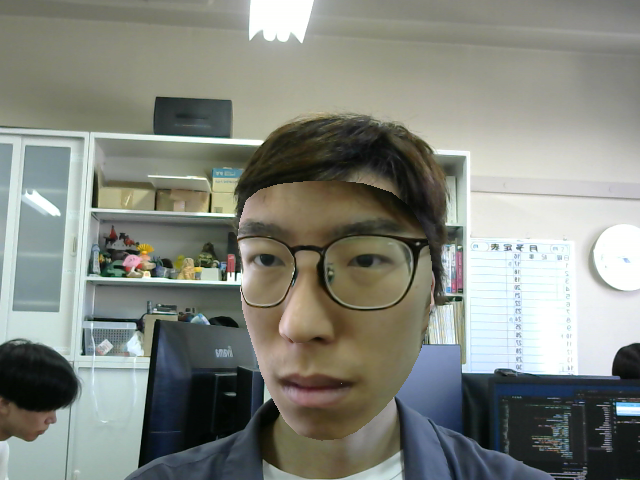
\includegraphics[keepaspectratio, scale=0.3]{figures/output5.png}
      \caption{実行結果(マスクあり)}
      \label{three}
    \end{minipage} &
    \begin{minipage}[t]{0.45\hsize}
      \centering
      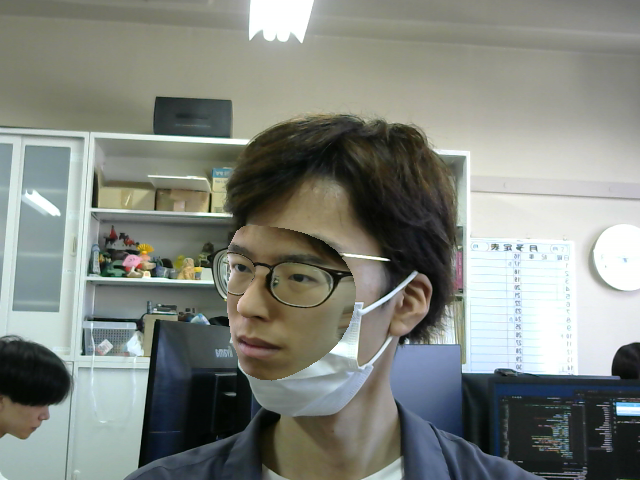
\includegraphics[keepaspectratio, scale=0.3]{figures/output6.png}
      \caption{実行結果(マスクあり)}
      \label{four}
    \end{minipage}
  \end{tabular}
\end{figure}
この結果から、顔が正面の角度の場合は、ある程度正確に表示できている事がわかる。
しかし顔に角度がある場合は、正しくモデルを貼り付けることができていない。これは顔認識モデルのFaceMeshがマスクをつけている場合
一定の角度以上で顔を認識することができないことが原因だと考えられる。
\section{夏休み中の進捗}
夏休み中には大きく分けて、オープンキャンパスの準備、別の顔認識モデルの利用、関連研究の調査の三点を進めた。以降の節ではそれぞれについて簡潔に報告する。

\subsection{オープンキャンバスの準備}
オープンキャンバスの準備として、簡素なGUIを作成した。GUIでは、表示するテクスチャを選択することができ、さまざまなテクスチャを基に三次元モデルを作成することで、
展示としての魅力を向上させた。\hyperref[five]{図\ref{five}}に作成したGUIを示す。
\begin{figure}[!ht]
 \begin{center}
    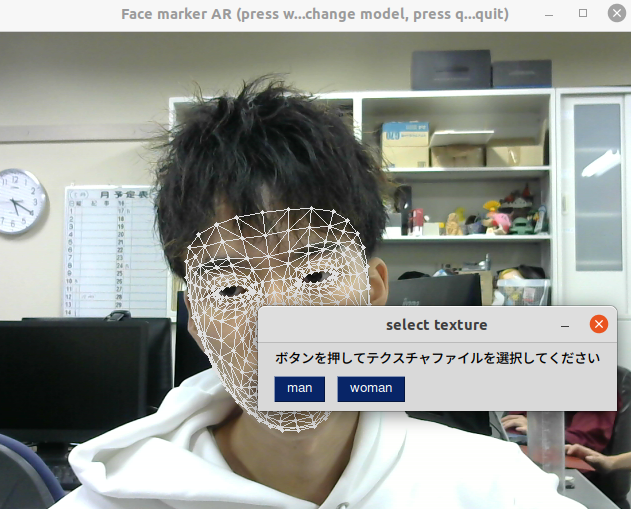
\includegraphics[scale=0.5]{figures/gui.png}
    \caption{GUI}
    \label{five}
  \end{center}
\end{figure}
\subsection{別の顔認識モデルの利用}
Google社が提供する顔認識モデルのうちの一つである、Mediapipe FaceDetectionを利用した。以前まで使用していたMediapipe FaceMeshと比較した利点として、全体として得る特徴点が少ないことによる、
動作の高速性がある。また、マスクをつけている場合でも、FaceMeshモデルと比較してある程度動作が安定するように感じた。欠点は二次元座標しか得られないことがあるが、
特徴点をカメラ姿勢の計算に利用する際、二次元座標をのみを用いているため、今回は問題ないと判断した。\\
現時点では、FaceMeshと同じように三次元モデルを貼りつけることはまだできていない。しかし、FaceMeshでは顔を認識できなかった角度についても、ある程度認識することができるので、
今後はFaceMeshと併用することも検討しつつ、研究を進めていきたい。
\subsection{関連研究の調査}
顔認識や、マスクを介したコミュニケーションなどの論文について査読した。\\
\hyperref[six]{図\ref{six}}はマスク着用時のコミュニケーションの印象の変化をまとめたものである。
論文\cite{bib_3}では、マスクをつけることで、顔の印象は平均化と悪化が同時に起こると示されている。
左の図では、顔の下半分が隠されることで、顔の印象の平均化が起きていることを示している。これは、顔の下半分の特徴が隠されてしまうことが原因であると推測される。
右の図では、マスクをつけることで、顔の印象が全体的に悪化することを示している。これは、マスクが不健康さを暗に示す事が原因であると推測される。
\begin{figure}[!ht]
  \begin{center}
     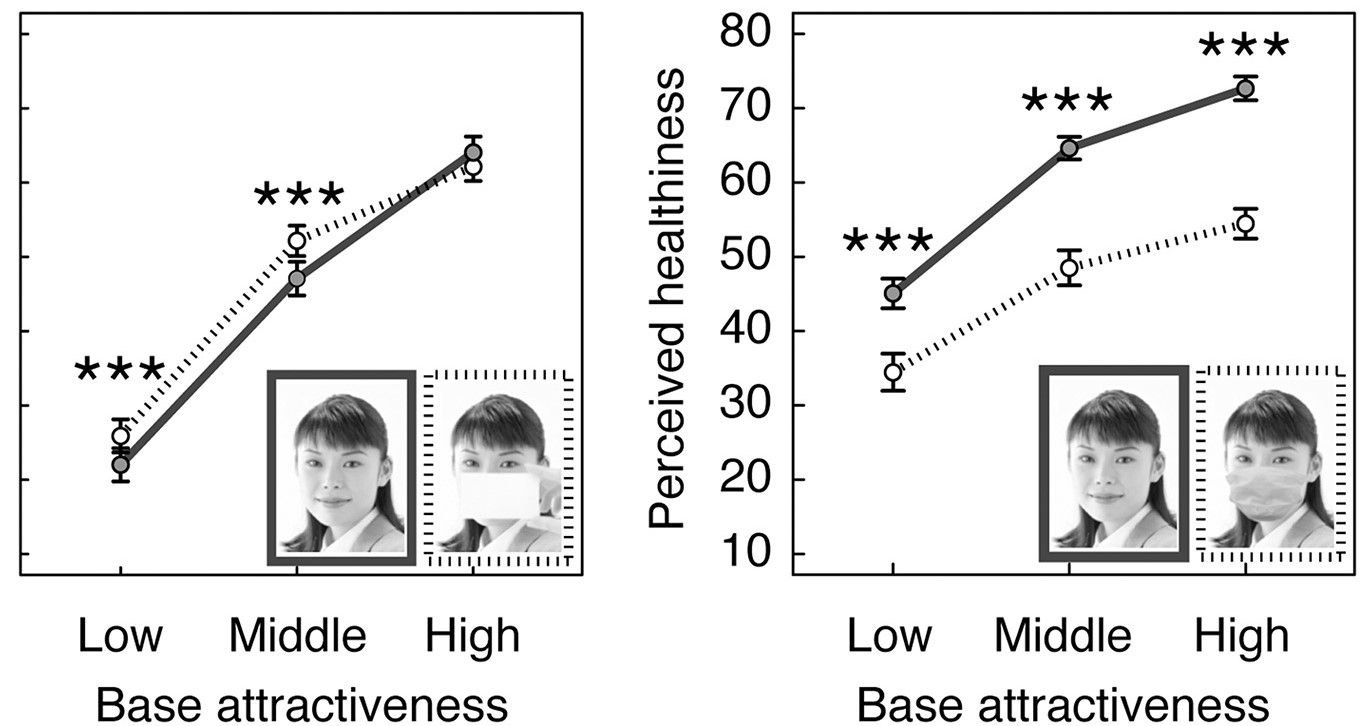
\includegraphics[scale=0.3]{figures/maskeffect.jpg}
     \caption{マスク着用によって顔の印象に与える効果}
     \label{six}
   \end{center}
 \end{figure}
\newpage
\section{後期の研究計画、目標}
後期の研究計画、目標について以下にまとめる。\\
10月~11月前半
\begin{itemize}
  \item より正確な顔の復元を行う。表情、モデルの輪郭処理、明度、色度、彩度の調整
  \item マスクを着用した状態で、顔の特徴点をより正しく、安定して取る方法を考える。別の顔認識モデルとの併用
\end{itemize}
11月前半~12月
\begin{itemize}
  \item 論文執筆開始
  \item マスクありの状態と比較して、コミュニケーション時の印象の変化を調査
\end{itemize}
%参考文献
\begin{thebibliography}{99}
\bibitem{bib_1} 菅谷保之,FaceMeshを利用した実寸サイズの3次元顔モデルの作成,閲覧日2023/7/26
\bibitem{bib_2} 中野学,Perspectibe-n-Point問題とその派生問題に対する安定かつ高速な解放に関する研究,閲覧日2023/7/26
\bibitem{bib_3} Yuki Miyazaki, Junichiro Kawahara, The sanitary mask effect on perceived facial attractiveness, pp.261-272, Figure 4,閲覧日2023/10/05
\end{thebibliography}

\end{document}
